% Options for packages loaded elsewhere
\PassOptionsToPackage{unicode}{hyperref}
\PassOptionsToPackage{hyphens}{url}
%
\documentclass[]{article}
\usepackage{ctex}
\usepackage{amsmath,amssymb}
\usepackage[table]{xcolor}
\usepackage{booktabs}
\usepackage{breqn}
\usepackage{multirow}

\begin{document}

后面我们通过生物种群相互竞争模型来预测未来几年的电动车与燃油车的数量关系。

\subsubsection{生物种群相互竞争模型}

当某个自然的环境中只有一种生物的群体(种群)生存时,我们常用Logistic模型来描述它的数量的演变过程,即:

\begin{dmath}
  x(t)=rx(1-\frac{x}{N})
\end{dmath}

如果一个自然环境中存在两个种群,它们之间的关系为相互竞争关系,并且数量变化服从Logistic规律。

于是我们对其中一种群甲有

\begin{dmath}
  x_1(t)=r_1x_1(1-\frac{x_1}{N_1})
\end{dmath}

这里因子(\(1-\frac{x_1}{N_1}\))反映由于甲对有限资源的消耗导致的对其自身增长的阻滞作用,$\frac{x_1}{N_1}$可理解为相对于$N_1$而言,数量为$x_1$时供养甲的食物量(设食物总量为单位量1)。

当考虑到甲乙两个种群在同一自然环境中生存时考虑到乙种群消耗统一资源对甲的增长的影响,我们的因子($1-\frac{x_1}{N_1}$)再减去一项,该项与种群乙的数量成正比,得到种群甲如下式:

\begin{dmath}x_1(t)=r_1x_1\left(1-\frac{x_1}{N_1}-\sigma_1\frac{x_2}{N_2}\right)\end{dmath}

上面$\sigma_1$
  表示单位数量的种群乙消耗的供养种群甲的食物量为单位数量甲消耗的供养甲的食物量的$\sigma_1$倍。$\sigma_2$则相反同理。

\subsubsection{本题模型建立}

回到本论文中,我们将电动汽车、燃油汽车与种群甲、乙作如下类比:

$x_1(t)$表示电动车在t时间的保有量,$x_2(t)$表示燃油车在t时间的保有量。

$r_1$、$r_2$分别表示电动车与燃油车的固有增长率。

$N_1$、$N_2$为电动车与燃油车的最大容量。

$\sigma_1$
  表示电动汽车相对于传统汽车在同等经济发展下的发展优势,$\sigma_2$
表示传统汽车对电动汽车同等经济发展下的发展优势。

首先我们假设其数量遵循Logistic规律,显然电动汽车与燃油汽车两者之间存在竞争关系,故我们利用生物种群相互竞争模型来预测未来几年的电动车与柴油车的数量关系。

得到如下方程:

\begin{dmath}
  \left\{
    \begin{aligned}
      x_1(t) & = r_1x_1(1-\frac{x_1}{N_1}-\sigma_1\frac{x_2}{N_2}) \\
      x_2(t) & = r_1x_2(1-\sigma_2\frac{x_1}{N_1}-\frac{x_2}{N_2})
    \end{aligned}
    \right.
\end{dmath}

$r_1$与$r_2$我们直接根据近年来两种汽车的增长情况求解得到,其中新能源车近年来固有增长率约为50\%(2022年中国新能源汽车行业市场前景及投资研究预测报告),燃油车近年来固有增长率约为4\%(杭州统计年鉴2021)。故取$r_1=0.5,r_2=0.04$。

$N_1$、$N_2$的确定存在不确定性,需要提前估算确定。由于电动汽车与燃油汽车的功能性基本相同,我们这里假设$N_1=N_2$。
对该值的估算方法普遍有三种,分别是直接选取最大值法、专家判断法和纯粹数学推导法。本研究采用专家判断法确定两种汽车最大保有量,根据文献(《我国到底能承载多少汽车?》------姜靖、戴慧兰),国家信息中心信息资源部主任徐长明认为,汽车保有量最高可达4.5亿辆。为了合理地预估我国个人汽车保有量极限,本论文中假设其极限占比为90\%,计算得出我国个人汽车最大保有量约为4.05亿辆。

$\sigma_1$ 与$\sigma_2$
的确定我们开创性地利用主成分分析法来得到主成分数据,以得到的主成分为自变量,汽车数量为因变量通过最小二乘法作线性回归,进而得到$\sigma_1$
  与$\sigma_2$。 方法如下。

\subsubsection{相关性分析}

通过对于以往研究电动汽车发展的论文,我们注意到影响我国电动汽车保有量变化的因素有多种,如经济因素,包括人均GDP、居民收入、经济产业结构、居民消费水平等;社会因素,包括城市人口、城市化率、失业率、拥塞成本等;环境因素,包括公路网规模、基础设施完善度等。考虑长期完整数据的可获得性,我们在这里初步选取了城市人口数、城市化水平、人均GDP、居民消费水平、公路里程、第一产业占比、第二产业占比、第三产业占比这8个代表性的影响因素进行分析。(数据大部分来源于《中国统计年鉴(2021)》)

首先我们将以上八个因素与电动汽车保有量进行了Spearman相关系数相关性分析,得到如下相关系数热力图。(电动汽车保有量来自于《2022年中国新能源汽车行业市场前景及投资研究预测报告》)

% \begin{figure}
%   \centering
%   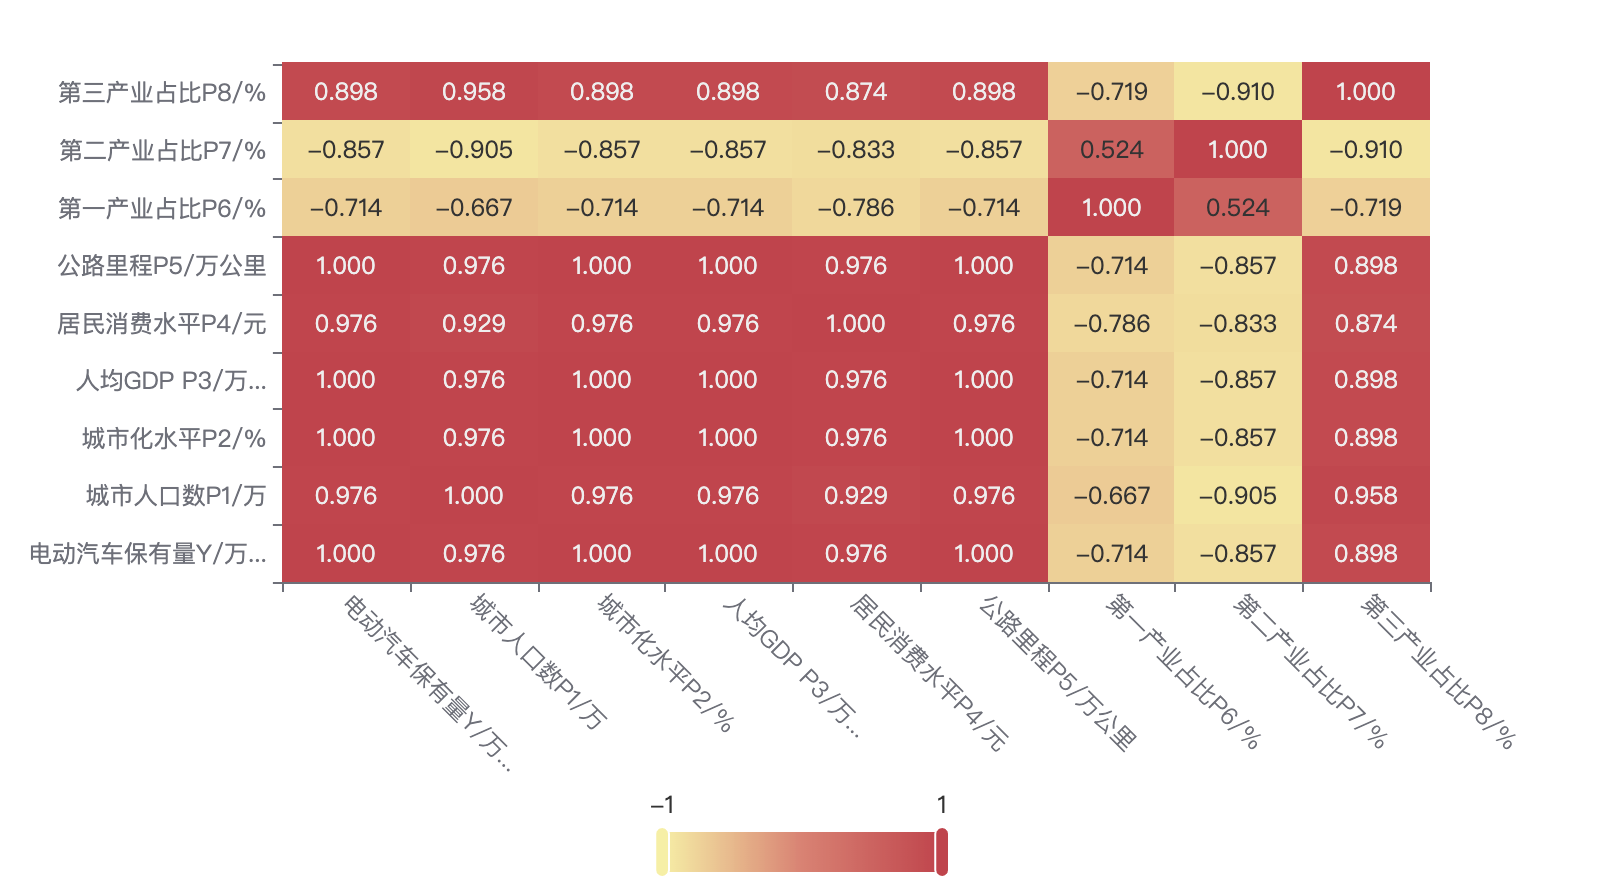
\includegraphics{/Users/younghol/Downloads/相关系数热力图 (2).png}
%   \caption{}
% \end{figure}

注意到第一产业占比、第二产业占比与电动汽车保有量相关性较低,所以我们在后续的主成分分析时略去这两种因素。

\subsubsection{{主成分分析}}

主成分分析法是运用``降维''思想,把多个指标变换成少数综合指标的多元统计方法,这里的综合指标就是主成分。每个主成分都是原始变量的线性组合,彼此相互独立,并保留了原始变量绝大部分信息。其本质是通过原始变量的相关性,寻求相关变量的综合替代对象,并且保证了转化过程中的信息损失最小
。

我们对城市人口数、城市化水平、人均GDP、居民消费水平、公路里程、第三产业占比六个因素通过SPSSPRO进行主成分分析,来综合评价每年度的社会经济发展水平。

(主成分分析的主要步骤\ldots\ldots 不知道要不要写,先省略)

KMO检验是 Kaiser, Meyer和 Olkin提出的抽样适合性检验( Measure of Sampling
Adequacy)。该检验是对原始变量之间的简相关系数和偏相关系数的相对大小进行检验。Bartlett球形度检验用于检验相关阵中各变量间的相关性,是否为单位阵,即检验各个变量是否各自独立。

我们得到KMO值=0.58,显著值p\textless0.001,水平上呈现显著性,拒绝原假设,各变量间具有相关性,主成分分析有效,效度虽然在0.6以下,但尚能接受。



\begin{table}[h]
  \centering
  \rowcolors{2}{white!20}{black!10}
  \setlength{\tabcolsep}{0.05\textwidth}{
  \begin{tabular}[]{llll}
    \toprule
    \rowcolor{blue!30}
    成分       & 特征根     &          &          \\
    特征根     & 方差百分比 & 累积     &          \\
    1          & 5.657      & 94.286\% & 94.286\% \\
    2          & 0.278      & 4.636\%  & 98.922\% \\
    3          & 0.056      & 0.927\%  & 99.849\% \\
    4          & 0.007      & 0.111\%  & 99.96\%  \\
    5          & 0.002      & 0.039\%  & 99.999\% \\
    6          & 0.000      & 0.001\%  & 100.0\%  \\
    \bottomrule
  \end{tabular}}
  \caption{总方差解释}
  \label{tab:总方差解释}
\end{table}


% \begin{figure}
%   \centering
%   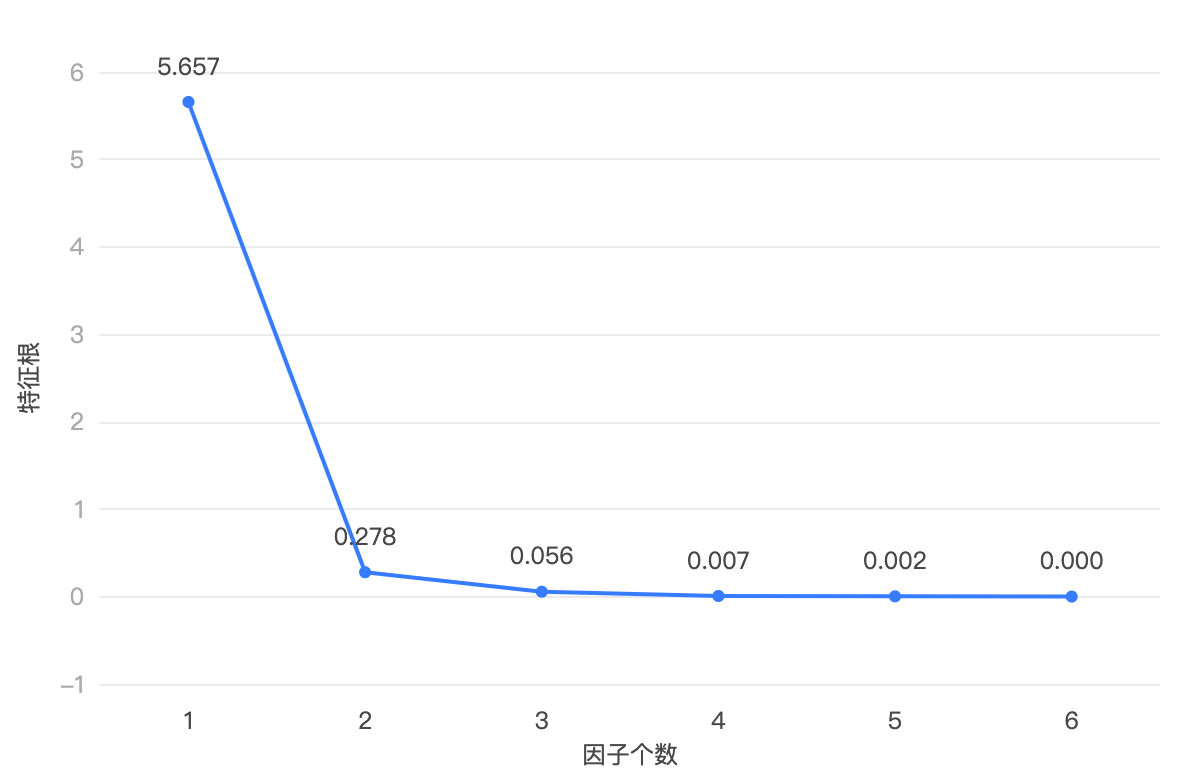
\includegraphics{/Users/younghol/Downloads/因子分析碎石图.png}
%   \caption{}
% \end{figure}

上面方差解释表中,我们发现第一主成分的特征值λ=5.657\textgreater1,,且远大于其他特征值,
累积方差贡献率为94.286\%,
即可以解释总体数据的94.286\%。由碎石图可知,在第二个主成分开始特征值下降坡度变缓,且前两个主成分累积解释贡献率超过90\%,因此我们选择两个主成分进行分析。

从下面的因子载荷矩阵热力图中可以分析每个主成分中隐变量的重要性,其中第一个主成分与前五个因素都具有较大的相关性(0.9以上),我们概括为``城市总体发展程度''。主成分2与第三产业占比的相关程度较大,可以概括为``服务业发展程度''。

% \begin{figure}
%   \centering
%   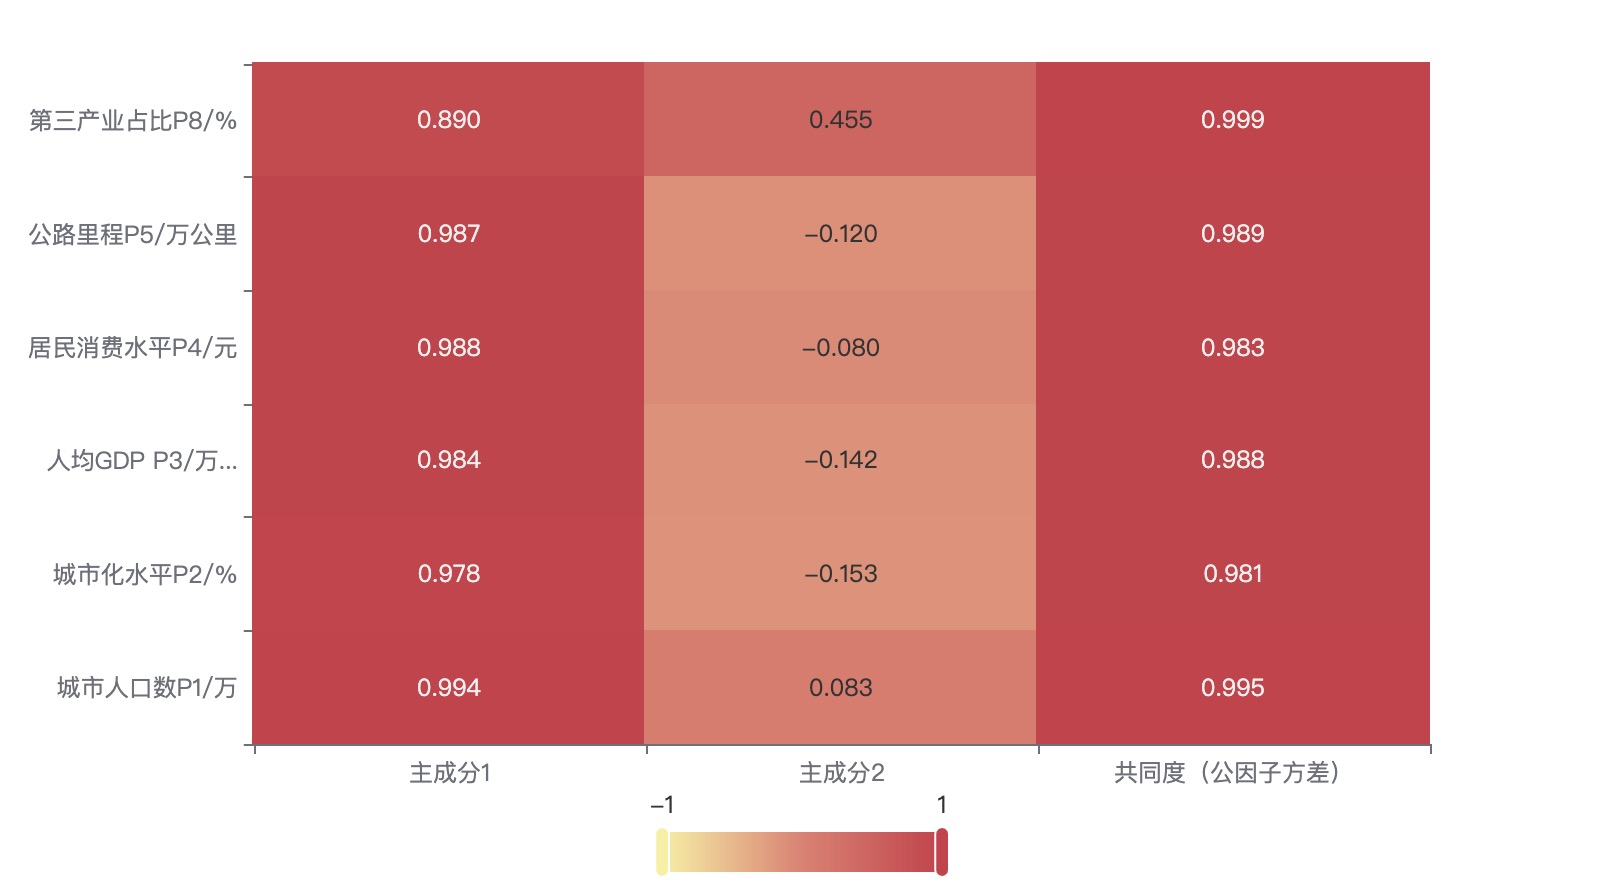
\includegraphics{/Users/younghol/Downloads/相关系数热力图 (3).png}
%   \caption{}
% \end{figure}

根据表\ref{tab:总方差解释}我们得到模型的公式:

\begin{dmath}
  F1=0.176\times\mbox{\bf 城市人口数}P1+0.173\times\mbox{\bf 城市化水平}P2+0.174\times\mbox{\bf 人均GDP}P3+0.175\times\mbox{\bf 居民消费水平}P4+0.174\times\mbox{\bf 公路里程}P5+0.157\times\mbox{\bf 第三产业占比}P8
\end{dmath}

\begin{dmath}
  F2=0.299\times\mbox{\bf 城市人口数}P1-0.549\times\mbox{\bf 城市化水平}P2-0.511\times\mbox{\bf 人均GDP}P3-0.289\times\mbox{\bf 居民消费水平}P4-0.433\times\mbox{\bf 公路里程}P5+1.635\times\mbox{\bf 第三产业占比}P8
\end{dmath}

由上可以得到:

\begin{dmath}
  F=(0.943/0.989)\times F1+(0.046/0.989)\times F2
\end{dmath}

\begin{table}[h]
  \centering
  \rowcolors{2}{white!20}{black!10}
  \setlength{\tabcolsep}{0.07\textwidth}{
  \begin{tabular}[]{lcc}
    \toprule
    \rowcolor{blue!30}
      &\multicolumn{2}{c}{成分}\\
    \rowcolor{blue!30}
       \multicolumn{1}{c}{名称}  &成分1 &  成分2\\
    城市人口数P1/万   & 0.176 & 0.299  \\
    城市化水平P2/\%   & 0.173 & -0.549 \\
    人均GDP P3/万元   & 0.174 & -0.511 \\
    居民消费水平P4/元 & 0.175 & -0.289 \\
    公路里程P5/万公里 & 0.174 & -0.433 \\
    第三产业占比P8/\% & 0.157 & 1.635  \\
    \bottomrule
  \end{tabular}}
  \caption{成分矩阵表}
  \label{tab:成分矩阵表}
\end{table}


由下图可知:第一主成分值与年份呈显著的线性正相关,
故利用线性回归模型得出第一主成分(y)与年份(x)的关系, 如式:

\begin{dmath}
  y=0.4071x-820.4
\end{dmath}

% \begin{figure}
%   \centering
%   \includegraphics{https://tkoghgi47p.feishu.cn/space/api/box/stream/download/asynccode/?code=NTY2MzY4ZDViMmU5N2JmOWU0ZmE5OTgyZGVhNmFhM2NfN0xrZVdBbjVJZ2VrVHpvU1N2NmdkdDNRVlM4VWxSdE9fVG9rZW46Ym94Y25yNUhGSEpnQjNQcmZUMGJTSUtJRDJBXzE2NTI5Mzg4NjM6MTY1Mjk0MjQ2M19WNA}
%   \caption{}
% \end{figure}

第一主成分与电动汽车、燃油汽车保有量均存在明显的非线性关系,
故考虑选取第一主成分为基准得到后面生物种群相互竞争模型中的$\sigma_1$
  、$\sigma_2$ 值。

\subsubsection{{线性回归(最小二乘法)}}

我们使用SPSSPRO,将得到的第一主成分值分别与电动汽车数量、燃油汽车数量作线性回归,得到如下拟合效果图。

% \begin{figure}
%   \centering
%   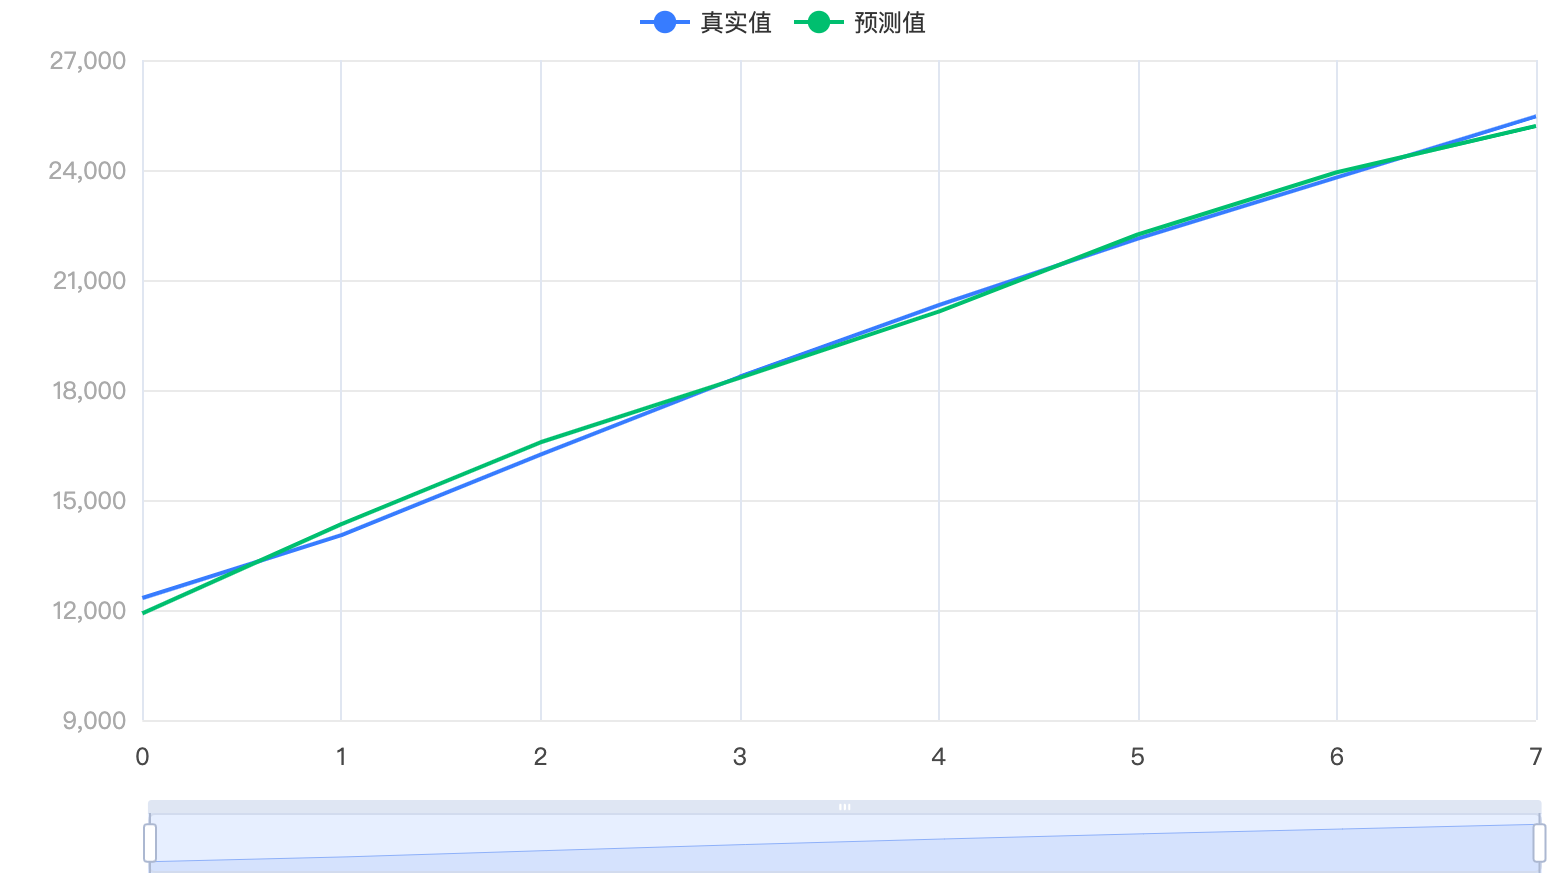
\includegraphics{/Users/younghol/Downloads/拟合效果图 (1).png}
%   \caption{}
% \end{figure}

% \begin{figure}
%   \centering
%   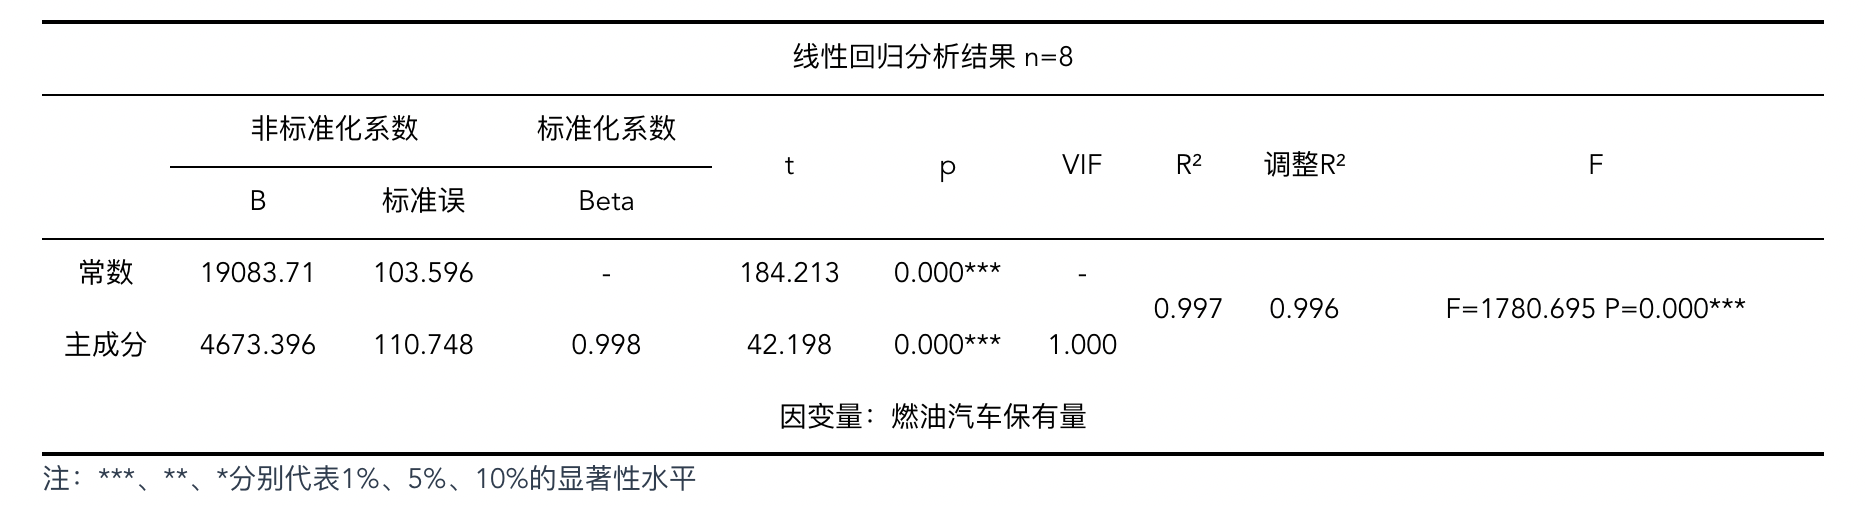
\includegraphics{/Users/younghol/Desktop/截屏2022-05-19 下午5.30.59.png}
%   \caption{}
% \end{figure}

燃油汽车保有量=19083.71+4673.396*主成分

% \begin{figure}
%   \centering
%   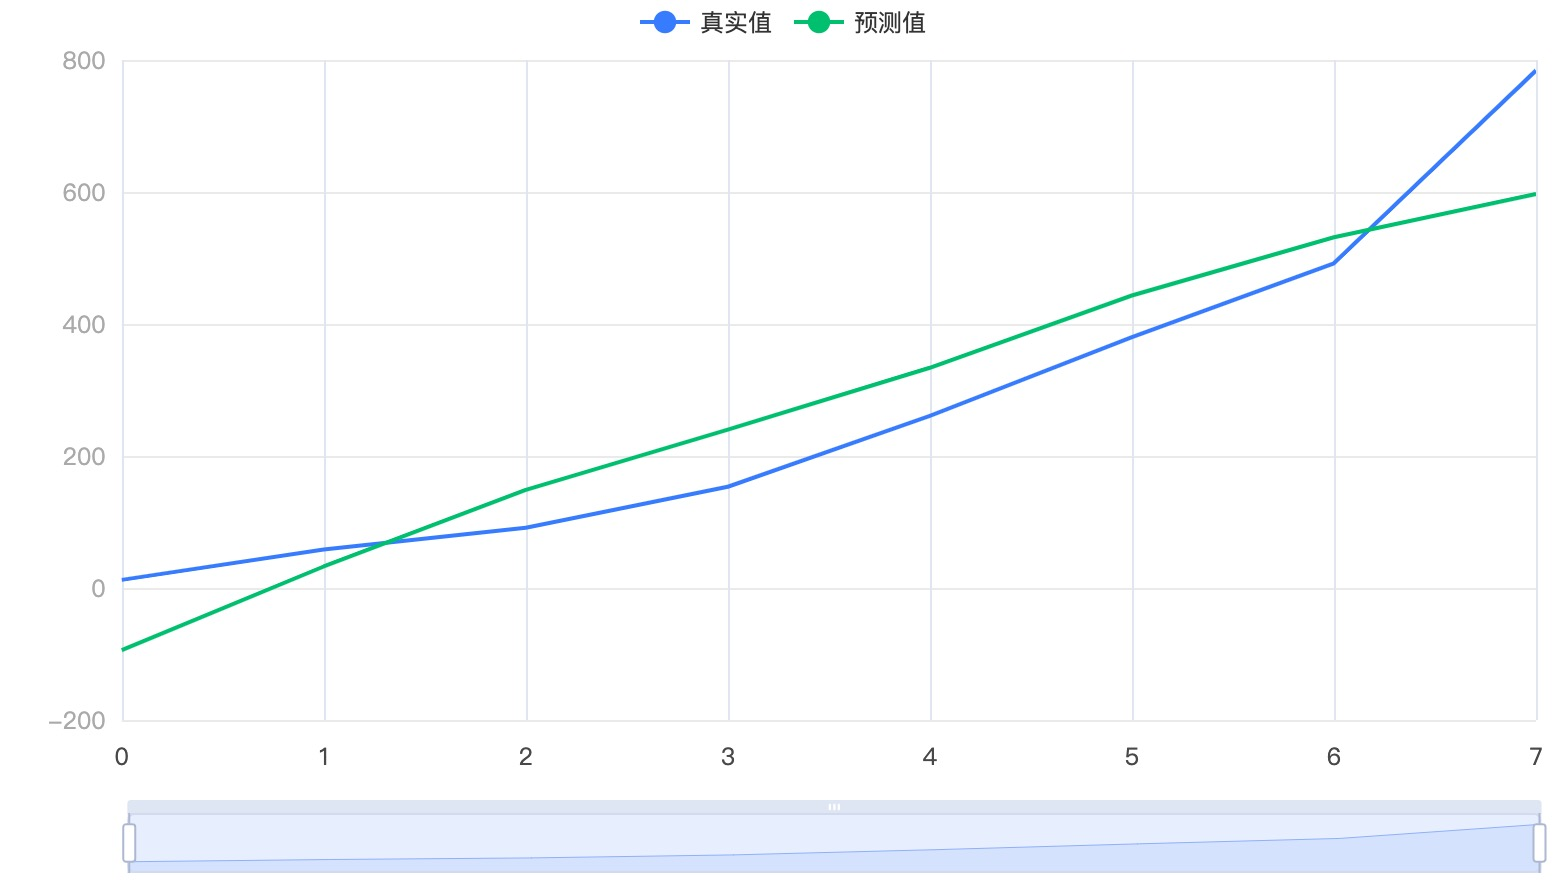
\includegraphics{/Users/younghol/Downloads/拟合效果图.png}
%   \caption{}
% \end{figure}

% \begin{figure}
%   \centering
%   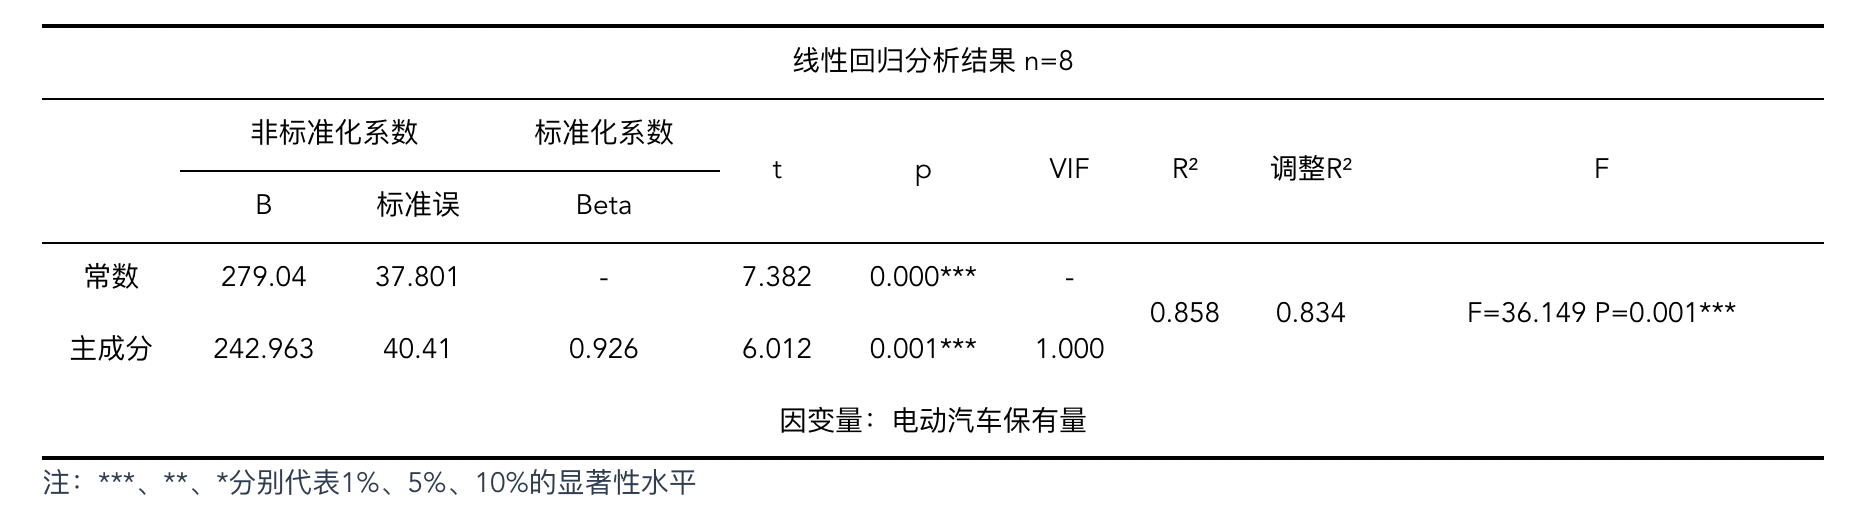
\includegraphics{/Users/younghol/Desktop/截屏2022-05-19 下午5.29.26.png}
%   \caption{}
% \end{figure}

电动汽车保有量=279.04+242.963*主成分

以上回归分析结果中,从F检验的结果分析可以得到,显著性P值均为0.000***,水平上呈现显著性,
拒绝回归系数为0的原假设,
因此模型基本满足要求对于变量共线性表现,VIF全部小于10,模型没有多重共线性问题,
模型构建良好 。

\begin{equation}
  \sigma_1=\frac{4673.396}{19083.71}\approx0.24
\end{equation}

\begin{equation}
  \sigma_2= \frac{242.963}{279.04} \approx0.87
\end{equation}

\subsubsection{模型的求解}

我们使用matlab对该生物种群相互竞争模型进行求解,得到如下结果:

% \begin{figure}
%   \centering
%   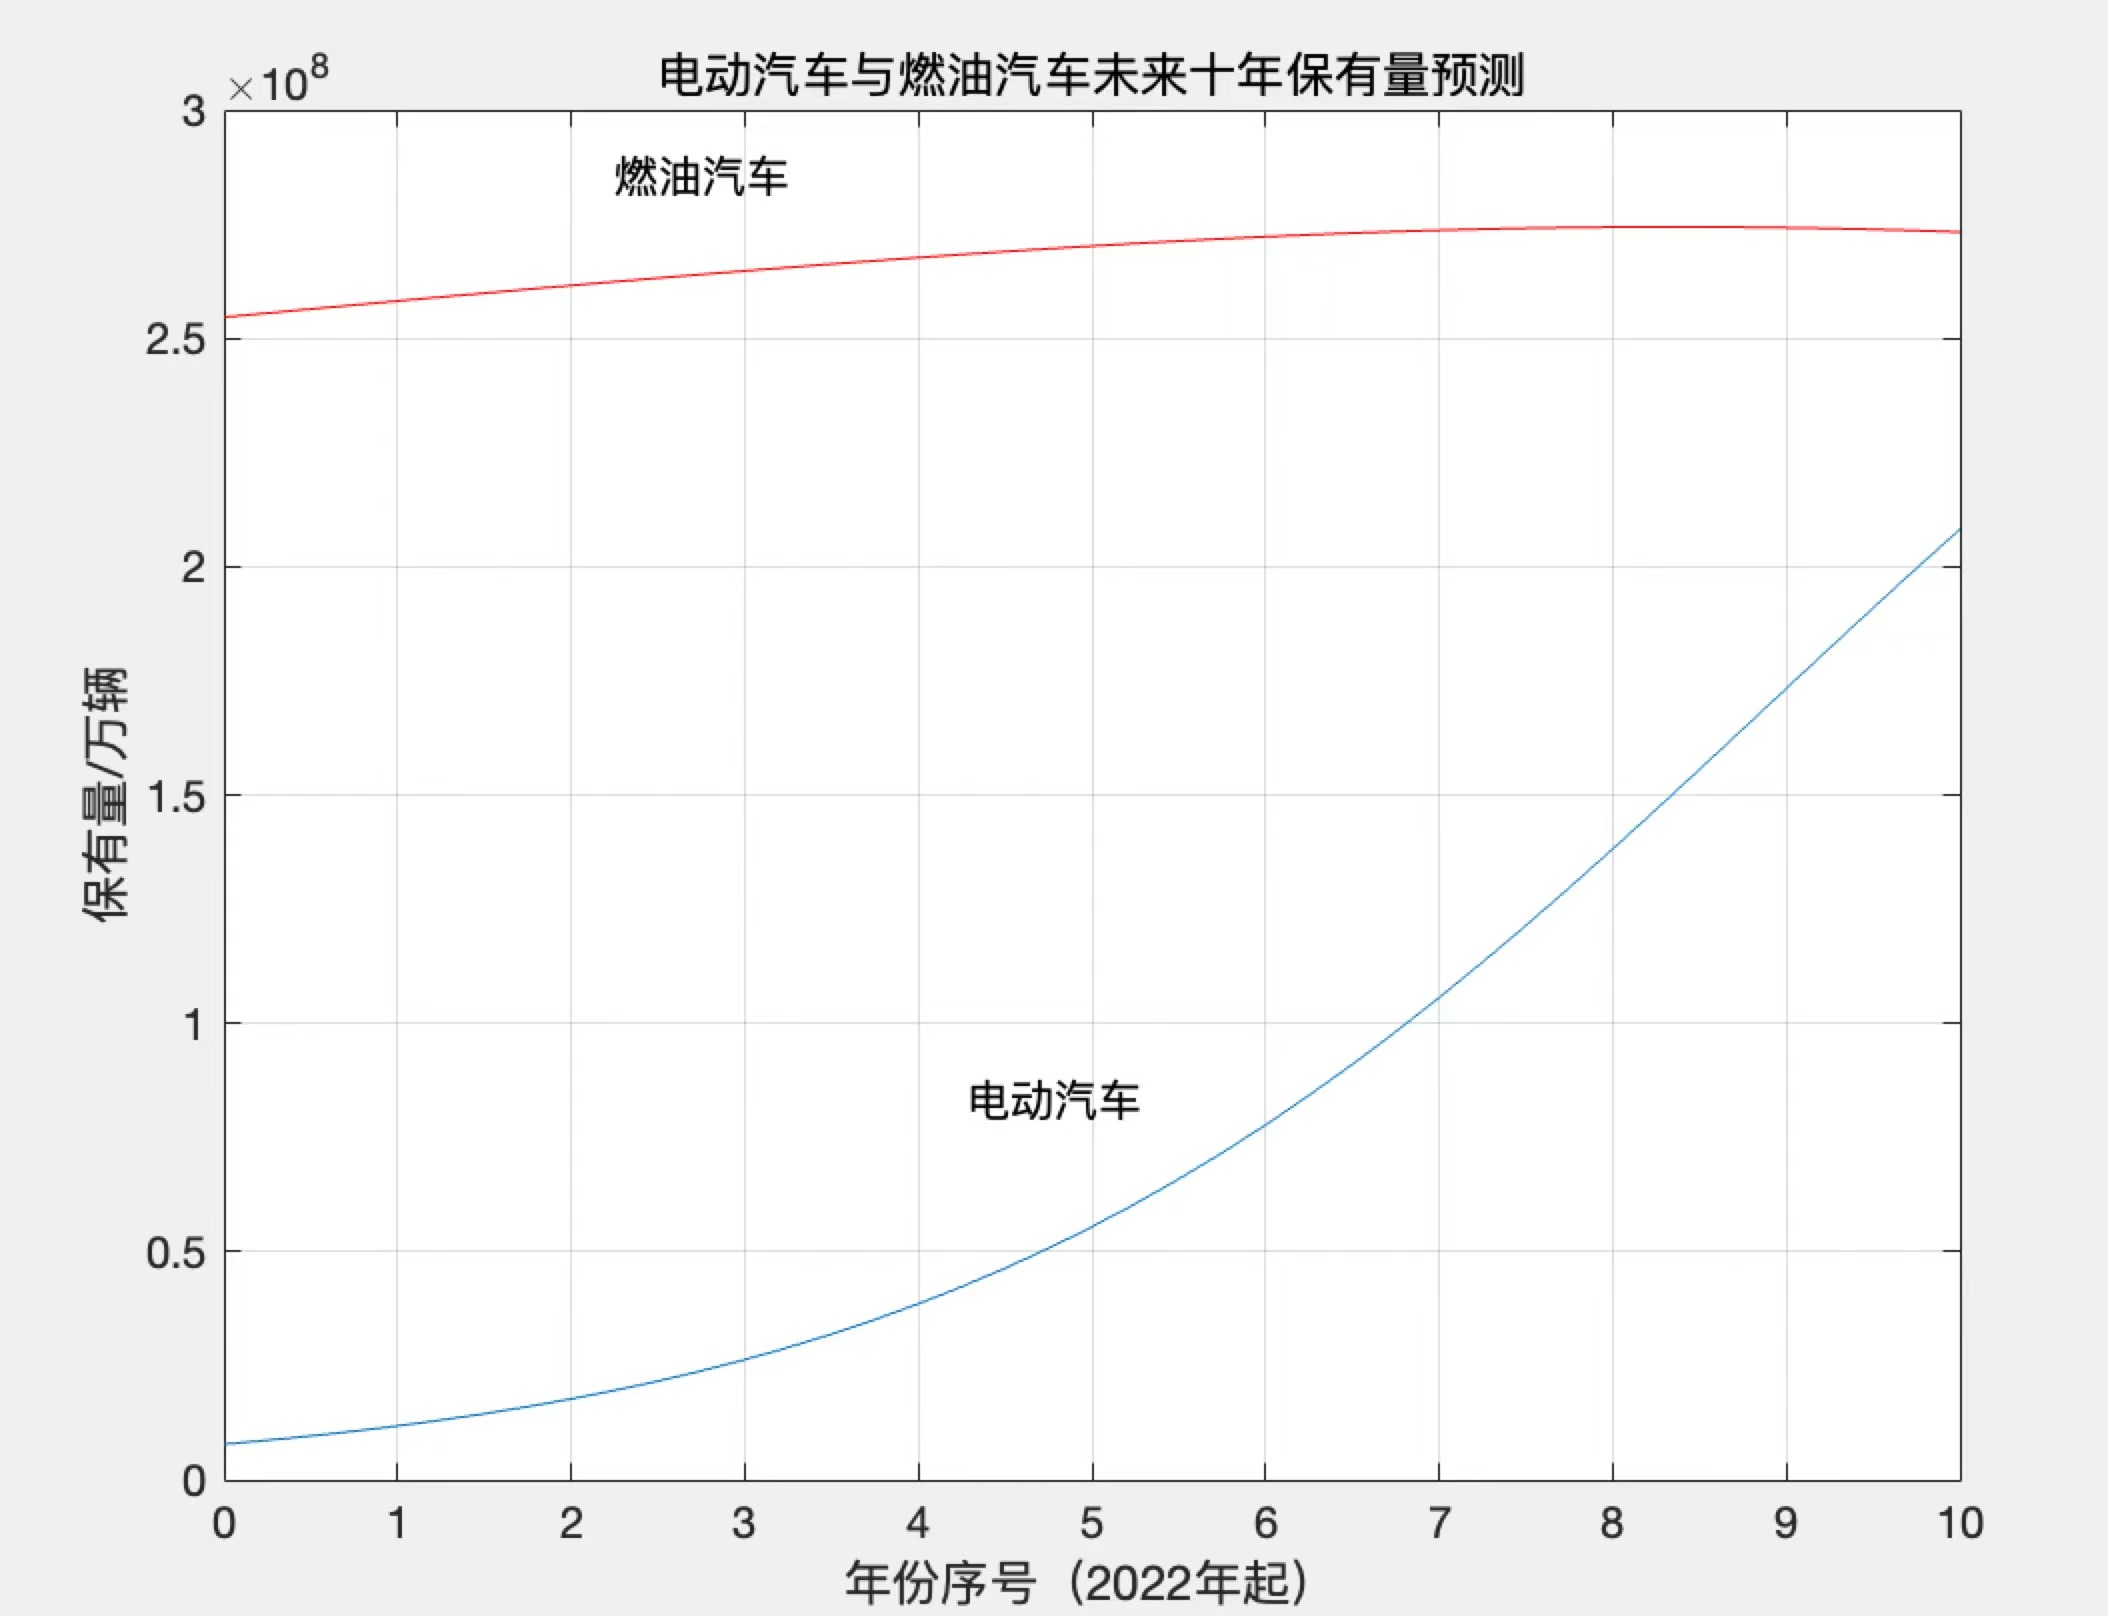
\includegraphics{/Users/younghol/Desktop/911652953505_.pic.jpg}
%   \caption{}
% \end{figure}

根据最新统计数据,2022年第一季度电动汽车保有量为891.5万辆,与我们预测的结果873.9万辆基本接近。

\end{document}
